% arara: latexmk: { engine: lualatex, options: [-synctex=1, -aux-directory=./build] }
\documentclass[polish,pretty]{angav}

\title{Lean \& ITP}
\author{Michał Dobranowski}
\date{\today}

\setmonofont{JetBrainsMono}[Scale=0.85,Contextuals=AlternateOff]  % disable ligatures

\usepackage{ebproof}
\usepackage{stmaryrd} % for \llbracket and \rrbracket
\newcommand{\toto}{\twoheadrightarrow}
\newcommand{\FV}{\opname{FV}}
\newcommand{\Lean}[1]{\mintinline[fontsize=\normalsize]{lean4}{#1}}
\newcommand{\centerLean}[2][]{\begin{center}\Lean{#2}#1\end{center}}

\begin{document}
\maketitle
\tableofcontents
\newpage

\section{Wstęp teoretyczny}

Aby zrozumieć, dlaczego systemowi wspomagającego dowodzenie (ang. \textit{proof assistant}) możemy ufać bardziej niż tuszowi na papierze, należy zrozumieć narzędzia oferowane przez logikę, rachunek lambda oraz teorię typów, na których zbudowany jest każdy znany autorowi tego typu system.
Chociaż ten kurs nigdy nie miał być teoretyczny, zdaniem autora formalizmy dotyczące (typowanego) rachunku lambda są niezwykle ciekawe, więc w odpowiednich miejscach Czytelnik jest zachęcany do pogłębienia wiedzy, w tym też przeprowadzenia lub przeczytania dowodów przytaczanych twierdzeń.

\subsection{Logika intuicjonistyczna}

Typowym przykładem ilustrującym różnicę między logiką klasyczną a intuicjonistyczną (konstruktywną) jest twierdzenie:
\begin{displayquote}
    Istnieją takie liczby niewymierne $a$ i $b$, że $a^b$ jest liczbą wymierną.
\end{displayquote}
oraz jego dowód:
\begin{displayquote}
    Jeśli $\sqrt{2}^{\sqrt{2}} \in \QQ$, to $a = b = \sqrt{2}$, w przeciwnym razie niech $a = \sqrt{2}^{\sqrt{2}}$ oraz $b = \sqrt{2}$, wtedy $a^b = 2 \in \QQ$.
\end{displayquote}
Dowód ten jest oczywiście słuszny na gruncie logiki klasycznej, ale nie jest konstruktywny, ponieważ dalej nie znamy odpowiednich liczb $a$ i $b$. W logice konstruktywnej zdanie jest prawdziwe, jeśli można podać jest \vocab{konstrukcję} (tzn. intuicyjny dowód), zgodnie z interpretacją Brouwera-Heytinga-Kolmogorowa:
\begin{itemize}[noitemsep]
    \item konstrukcja dla $A \land B$ to konstrukcja dla $A$ oraz konstrukcja dla $B$,
    \item konstrukcja dla $A \lor B$ to konstrukcja dla $A$ lub konstrukcja dla $B$ wraz z zaznaczeniem, która z nich to jest,
    \item konstrukcja dla $A \to B$ to przekształcenie każdej konstrukcji dla $A$ w konstrukcję dla $B$,
    \item nie istnieje konstrukcja dla fałszu.
\end{itemize}

Formalnie, logika intuicjonistyczna to pewien system logiczny. Nie różni się od logiki klasycznej składnią, ale regułami wnioskowania.
Fałsz oznaczamy przez $\bot$, a \vocab{osąd} zapisany w postaci $\Gamma \vdash A$ oznacza, że formuła $A$ wynika ze zbioru formuł (założeń) $\Gamma$.
Zamiast $\Gamma \cup \{B\}$ będziemy często pisać $\Gamma, B$.

\begin{figure}[H]
    \[
    \begin{prooftree}
        \infer0[(Ax)]{\Gamma,A\vdash A}
    \end{prooftree}
    \qquad
    \begin{prooftree}
        \hypo{\Gamma\vdash \bot}
        \infer1[($\bot\!$ E)]{\Gamma\vdash A}
    \end{prooftree}
    \]

    \[
    \begin{prooftree}
        \hypo{\Gamma\vdash A}
        \hypo{\Gamma\vdash B}
        \infer2[($\land\!$ I)]{\Gamma\vdash A \land B}
    \end{prooftree}
    \qquad
    \begin{prooftree}
        \hypo{\Gamma\vdash A \land B}
        \infer1[($\land\!$ E1)]{\Gamma\vdash A}
    \end{prooftree}
    \qquad
    \begin{prooftree}
        \hypo{\Gamma\vdash A \land B}
        \infer1[($\land\!$ E2)]{\Gamma\vdash B}
    \end{prooftree}
    \]

    \[
    \begin{prooftree}
        \hypo{\Gamma\vdash A}
        \infer1[($\lor\!$ I1)]{\Gamma\vdash A \lor B}
    \end{prooftree}
    \qquad
    \begin{prooftree}
        \hypo{\Gamma\vdash A}
        \infer1[($\lor\!$ I2)]{\Gamma\vdash B \lor A}
    \end{prooftree}
    \qquad
    \begin{prooftree}
        \hypo{\Gamma\vdash A \lor B}
        \hypo{\Gamma,A\vdash C}
        \hypo{\Gamma,B\vdash C}
        \infer3[($\lor\!$ E)]{\Gamma\vdash C}
    \end{prooftree}
    \]

    \[
    \begin{prooftree}
        \hypo{\Gamma,A\vdash B}
        \infer1[($\to\!$ I)]{\Gamma\vdash A \to B}
    \end{prooftree}
    \qquad
    \begin{prooftree}
        \hypo{\Gamma\vdash A \to B}
        \hypo{\Gamma\vdash A}
        \infer2[($\to\!$ E)]{\Gamma\vdash B}
    \end{prooftree}
    \]
    \caption{Reguły wnioskowania w intuicjonistycznym rachunku zdań (IRZ).}
\end{figure}

Oprócz tego, definiujemy negację jako $\neg A \coloneqq A \to \bot$. Dzięki tej definicji oraz regule ($\to\!$~E) możemy wywieść
\[
\begin{prooftree}
    \hypo{\Gamma\vdash A}
    \hypo{\Gamma\vdash \neg A}
    \infer2[($\neg\!$ E)]{\Gamma\vdash \bot}
\end{prooftree}
\]
Oznaczamy również prawdę przez $\top \coloneqq \neg\bot = \bot \to \bot$.

\begin{example}
    Pokaż, że w IRZ zachodzi \vocab{słabe prawo podwójnej negacji}, czyli $A \to \neg\neg A$.
\end{example}
\begin{solution}
    Z definicji negacji mamy $\neg\neg A = (A \to \bot) \to \bot$, więc musimy pokazać $A \to ((A\to\bot) \to \bot)$.
    \[
    \begin{prooftree}
        \infer0[(Ax)]{A, A\to\bot \vdash A\to\bot}
        \infer0[(Ax)]{A, A\to\bot \vdash A}
        \infer2[($\to\!$ E)]{A, A\to\bot \vdash \bot}
        \infer1[($\to\!$ I)]{A \vdash (A\to\bot) \to \bot}
        \infer1[($\to\!$ I)]{\vdash A \to ((A\to\bot) \to \bot)}
    \end{prooftree}
    \]
\end{solution}

\begin{example}
    Pokaż, że w IRZ zachodzi \vocab{prawo kontrapozycji}, czyli $(A \to B) \to (\neg B \to \neg A)$.
\end{example}
\begin{solution}
    Z definicji negacji mamy $\neg B = B \to \bot$ oraz $\neg A = A \to \bot$, więc musimy pokazać $(A \to B) \to ((B\to\bot) \to (A\to\bot))$.
    \[
    \resizebox{\hsize}{!}{
    \begin{prooftree}
        \infer0[(Ax)]{A\to B, B \to \bot, A \vdash B \to \bot}
        \infer0[(Ax)]{A\to B, B \to \bot, A \vdash A \to B}
        \infer0[(Ax)]{A\to B, B \to \bot, A \vdash A}
        \infer2[($\to\!$ E)]{A \to B, B \to \bot, A \vdash B}
        \infer2[($\to\!$ E)]{A \to B, B \to \bot, A \vdash \bot}
        \infer1[($\to\!$ I)]{A \to B, B \to \bot \vdash A\to\bot}
        \infer1[($\to\!$ I)]{A \to B \vdash (B \to \bot) \to (A \to \bot)}
        \infer1[($\to\!$ I)]{\vdash (A \to B) \to ((B \to \bot) \to (A \to \bot))}
    \end{prooftree}
    }
    \]
\end{solution}

\subsubsection{Związek z logiką klasyczną}

Dokładając do reguł wnioskowania IRZ \vocab{silne prawo podwójnej negacji} ($\neg\neg A \to A$) lub \vocab{prawo wyłączonego środka} ($A \lor \neg A$),  otrzymujemy logikę klasyczną.
W przypadku prawa podwójnej negacji jest to oczywiste. W przypadku prawa wyłączonego środka (EM) można to pokazać następująco:
\[
\resizebox{\hsize}{!}{
\begin{prooftree}
    \infer0[(\textcolor{AccColor1}{EM})]{(A \to \bot) \to \bot \vdash A \lor (A \to \bot)}
    \infer0[(Ax)]{(A \to \bot) \to \bot, A \vdash A}
    \infer0[(Ax)]{\Gamma \vdash (A \to \bot) \to \bot}
    \infer0[(Ax)]{\Gamma \vdash A \to \bot}
    \infer2[($\to\!$ E)]{\Gamma \vdash \bot}
    \infer1[($\bot\!$ E)]{\Gamma \vdash A}
    \infer3[($\lor\!$ E)]{(A \to \bot) \to \bot \vdash A}
    \infer1[($\to\!$ I)]{\vdash (A \to \bot) \to \bot \to A}
\end{prooftree}
}
\]
gdzie $\Gamma = \{(A \to \bot) \to \bot, A \to \bot\}$.

\begin{problem}
    Pokazać, że prawo wyłączonego środka nie jest dowodliwe w IRZ.
\end{problem}

\begin{remark*}[ciekawostka]
    Istnieją tautologie KRZ, które nie są dowodliwe w IRZ, ale po dodaniu do IRZ jako aksjomaty nie prowadzą do logiki klasycznej, tworząc logiki \enquote{pomiędzy} intuicjonistyczną i klasyczną. Przykłady:
    \begin{itemize}
        \item IRZ + $(\neg A \lor \neg\neg A)$\footnote{słabe prawo wyłączonego środka} --- logika Jankova (de Morgana), w której zachodzą wszystkie cztery prawa de Morgana,
        \item IRZ + $((A \to B) \lor (B \to A))$ --- logika Gödla-Dummeta, w której wartościowania formuł można interpretować jako liczby z przedziału $[0,1]$.
    \end{itemize}
\end{remark*}

Skoro zbiór reguł wnioskowania IRZ jest podzbiorem zbioru reguł wnioskowania KRZ, to każda formuła dowodliwa IRZ jest również dowodliwa w KRZ.

\subsubsection{Semantyka}

Trochę zaniedbując formalizmy, skupimy się przez chwilę na wartościowaniach formuł logicznych.
Możemy określić \vocab{semantykę} dla logiki klasycznej, przypisując formułom prawdziwym wartość $1$, a formułom fałszywym wartość $0$ (definiując przy okazji funkcje $\land, \lor, \to$).
Dla logiki intuicjonistycznej jest to trudniejsze, ale i ciekawsze. Pokażemy dwa z (nieskończenie) wielu możliwych sposobów.
Oba z nich są \vocab{algebrami Heytinga}, których nie będziemy tutaj definiować.
Warto jednak wiedzieć, że formuła logiczna jest tautologią IRZ wtedy i tylko wtedy, gdy jest prawdziwa w każdej algebrze Heytinga.

\paragraph{Semantyka topologiczna}
Możemy zdefiniować semantykę za pomocą topologii na $\RR$:
\begin{align*}
    \llbracket \bot \rrbracket &= \emptyset, \\
    \llbracket \top \rrbracket &= \RR, \\
    \llbracket A \land B \rrbracket &= \llbracket A \rrbracket \cap \llbracket B \rrbracket, \\
    \llbracket A \lor B \rrbracket &= \llbracket A \rrbracket \cup \llbracket B \rrbracket, \\
    \llbracket A \to B \rrbracket &= \opname{int}\left(\llbracket A \rrbracket^\complement \cup \llbracket B \rrbracket\right), \\
    \llbracket A \rrbracket &= \text{dowolny otwarty podzbiór $\RR$.}
\end{align*}
Wtedy
\[ \llbracket \neg A \rrbracket = \llbracket A \to \bot \rrbracket = \opname{int}\left(\llbracket A \rrbracket^\complement \cup \emptyset\right) = \opname{int}\left(\llbracket A \rrbracket^\complement\right) \]

Można przy pomocy takiej semantyki pokazać, że prawo wyłączonego środka nie jest dowodliwe w IRZ. Pod $\llbracket A \rrbracket$ możemy podstawić np. zbiór $(0, \infty)$, wtedy
\[ \llbracket A \lor \neg A \rrbracket = \llbracket A \rrbracket \cup \llbracket \neg A \rrbracket = \llbracket A \rrbracket \cup \opname{int}\left(\llbracket A \rrbracket^\complement\right) = (0, \infty) \cup (-\infty, 0) \neq \RR \]

\paragraph{Semantyka kraty dystrybutywnej}
Krata to zbiór częściowo uporządkowany, w którym istnieją kresy dolne i górne dowolnych par elementów.
Będziemy je przedstawiać za pomocą \vocab{diagramów Hassego}\footnote{Czym dokładnie jest diagram Hassego można dowiedzieć się na \href{https://pl.wikipedia.org/wiki/Diagram_Hassego}{Wikipedii}.}.
Definiujemy działania
\begin{align*}
    a \land b &\coloneqq \inf\{a, b\}, \\
    a \lor b &\coloneqq \sup\{a, b\}.
\end{align*}

Krata dystrybutywna to krata, w której zachodzą prawa rozdzielności:
\begin{align*}
    a \land (b \lor c) &= (a \land b) \lor (a \land c), \\
    a \lor (b \land c) &= (a \lor b) \land (a \lor c).
\end{align*}

Można udowodnić, że każda niepusta i skończona krata jest ograniczona, czyli posiada elementy najmniejszy i największy. Krata, która jest niepusta, skończona i dystrybutywna posłuży nam do zdefiniowania semantyki:
\begin{align*}
    \llbracket \bot \rrbracket &= \text{element najmniejszy}, \\
    \llbracket \top \rrbracket &= \text{element największy}, \\
    \llbracket A \land B \rrbracket &= \llbracket A \rrbracket \land \llbracket B \rrbracket, \\
    \llbracket A \lor B \rrbracket &= \llbracket A \rrbracket \lor \llbracket B \rrbracket, \\
    \llbracket A \to B \rrbracket &= \sup\{c : c \land \llbracket A \rrbracket \leq \llbracket B \rrbracket\}, \\
    \llbracket A \rrbracket &= \text{dowolny element kraty.}
\end{align*}
Wtedy
\[ \llbracket \neg A \rrbracket = \llbracket A \to \bot \rrbracket = \sup\{c : c \land \llbracket A \rrbracket \leq \llbracket \bot \rrbracket\} = \sup\{c : c \land \llbracket A \rrbracket = \llbracket \bot \rrbracket\} \]

Biorąc przykładową kratę
\begin{figure}[H]
    \centering
    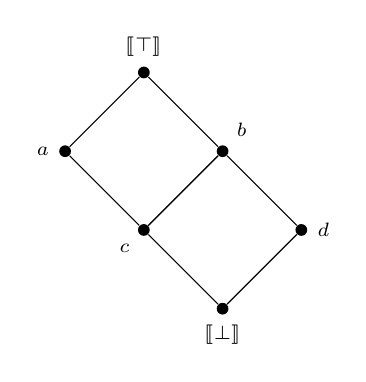
\begin{tikzpicture}[scale=2]
        \tikzset{dot/.style={circle, fill, inner sep=1.5pt}}
        \tikzset{every label/.append style={font=\scriptsize}}

        \node[dot,label=left:$a$]         (B) at (-0.5,0.5) {};
        \node[dot,label=above:$\llbracket \top \rrbracket$] (D) at (0,1) {};
        \node[dot,label=above right:$b$]  (C) at (0.5,0.5) {};
        \node[dot,label=below left:$c$]   (A) at (0,0) {};
        \node[dot,label=right:$d$]        (E) at (1,0) {};
        \node[dot,label=below:$\llbracket \bot \rrbracket$] (F) at (0.5,-0.5) {};

        \draw (B) -- (D) -- (C) -- (A) -- (B);
        \draw (A) -- (C) -- (E) -- (F) -- (A);
    \end{tikzpicture}
\end{figure}
możemy udowodnić, że prawo wyłączonego środka nie jest dowodliwe w IRZ. Jeśli weźmiemy $\llbracket A \rrbracket = c$, to $\llbracket \neg A \rrbracket = d$, więc $\llbracket A \lor \neg A \rrbracket = c \lor d = b \neq \llbracket \top \rrbracket$.

\begin{problem}
    Pokazać, że silne prawo podwójnej negacji nie jest dowodliwe w IRZ na podstawie dwóch powyższych semantyk.
\end{problem}

\begin{problem}
    Stwierdzić, które z czterech praw de Morgana są dowodliwe w IRZ.
\end{problem}

\subsection{Rachunek lambda}

Rachunek lambda to język złożony z termów, z których każdy to:
\begin{itemize}
    \item zmienna (zazwyczaj oznaczana małą literą, np. $x$),
    \item $\lambda$-abstrakcja postaci $\lambda x\ldotp M$, gdzie $x$ jest zmienną, a $M$ jest termem,
    \item aplikacja postaci $MN$, gdzie $M$ i $N$ są termami.
\end{itemize}

Formalnie termy można więc zdefiniować następująco:
\[ M \Coloneqq x \mid \lambda x\ldotp M \mid (MM), \]
gdzie $x$ reprezentuje dowolną zmienną.

Aby uprościć zapis, będziemy pisać $MNP$ zamiast $(MN)P$ -- to znaczy stwierdzamy, że aplikacja jest łączna lewostronnie. Ponadto, wiele $\lambda$-abstrakcji zapisujemy jako $\lambda x_1 \ldots x_n\ldotp M$, co jest równoważne termowi $\lambda x_1\ldotp (\lambda x_2\ldotp (\ldots (\lambda x_n\ldotp M) \ldots))$. Kropka w tym zapisie jest bardzo istotna, np.
\begin{align*}
    \lambda xyz\ldotp M &= \lambda x\ldotp (\lambda y\ldotp (\lambda z\ldotp M)), \\
    \lambda xy\ldotp z M &= \lambda x\ldotp (\lambda y\ldotp (z M)).
\end{align*}

W termie $\lambda x\ldotp M$ zmienna $x$ jest \vocab{zmienną związaną} w $M$.
Zmienne występujące w $M$, które nie są związane przez żadną $\lambda$-abstrakcję, nazywamy \vocab{zmiennymi wolnymi}.
Na przykład w termie $\lambda x\ldotp (x y)$ zmienna $x$ jest zmienną związaną, a $y$ jest zmienną wolną.
W termie $xz(\lambda xy\ldotp (xyz))$ zmienna $x$ raz występuje jako zmienna wolna, a raz jako związana. Takich sytuacji będziemy unikać ze względów czysto estetycznych.

Zbiór zmiennych wolnych termu $M$ oznaczamy jako $\FV(M)$.
Term nazywamy \vocab{termem zamkniętym} lub \vocab{kombinatorem}, jeśli $\FV(M) = \emptyset$.

\begin{remark}
    Formalnie definiujemy $\FV(M)$ rekurencyjnie:
    \begin{align*}
        \FV(x) &= \{x\}, \\
        \FV(\lambda x\ldotp M) &= \FV(M) \setminus \{x\}, \\
        \FV(MN) &= \FV(M) \cup FV(N).
    \end{align*}
\end{remark}

\subsubsection*{Alfa-konwersja}

\vocab{$\alpha$-konwersja} to przekształcenie termu, które polega na zmianie nazwy zmiennej (unikając kolizji oznaczeń zmiennych). Wprowadzamy relację równoważności $\equiv_\alpha$ w zbiorze termów $\Lambda$ w ten sposób, że dane dwa termy $M$ i $N$ są równoważne, jeśli można otrzymać jeden z drugiego poprzez (wielokrotne) $\alpha$-konwersje. Na przykład:
\[ a (\lambda b\ldotp bc) \equiv_\alpha a (\lambda d\ldotp dc), \]
natomiast
\[ \lambda a\ldotp ab \nequiv_\alpha \lambda b\ldotp bb, \]
ponieważ zamiana zmiennej $a$ na $b$ prowadzi do kolizji oznaczeń zmiennych.

Od tej pory utożsamiamy ze sobą termy różniące się jedynie nazwami zmiennych, czyli jeśli $M \equiv_\alpha N$, to $M$ i $N$ są tym samym termem.

\begin{remark}
    Bardziej formalnie, od tej pory będziemy operować na klasach abstrakcji relacji $\equiv_\alpha$ (elementach zbioru $\Lambda/{\equiv_\alpha}$), podobnie jak przy działaniach modulo operujemy na klasach abstrakcji relacji przystawania modulo $p$ (elementach zbioru $\ZZ/{\equiv_p}$).
\end{remark}

Będziemy stosować dosyć uniwersalny zapis $M[x \coloneqq N]$ na term, który powstał z termu $M$ poprzez zastąpienie wszystkich \emph{wolnych} wystąpień zmiennej $x$ termem $N$.
Zakładamy przy tym, że żadna zmienna wolna w $N$ nie zacznie być związana w $M[x \coloneqq N]$ (ponownie unikamy kolizji oznaczeń).

\subsubsection*{Beta-redukcja}

\vocab{$\beta$-redukcja} to taka relacja $\to_\beta$ w zbiorze termów $\Lambda$, że $M \to_\beta N$, gdy \vocab{$\beta$-redeks} postaci $(\lambda x\ldotp P)Q$ w termie $M$ zostaje zastąpiony przez $P[x \coloneqq Q]$ w termie $N$.
Relacja $\toto_\beta$ to domknięcie przechodnio-zwrotne relacji $\to_\beta$ (czyli najmniejsza relacja przechodnia i zwrotna, która zawiera relację $\to_\beta$), a $=_\beta$ to jej domknięcie równoważnościowe.
Piszemy $M \downarrow_\beta N$, jeśli istnieje term $P$ taki, że $M \toto_\beta P$ i $N \toto_\beta P$.

Jeśli w termie występuje więcej niż jeden $\beta$-redeks, to $\beta$-redukcja nie jest deterministyczna -- możemy wybrać dowolny z nich i wykonać redukcję.

\begin{example}
    \label{eq:beta-reduction}
    Pokazane poniżej są niektóre ścieżki redukcyjne dla podanego termu.
    \tikzset{>={Computer Modern Rightarrow[scale=1.3]}}
    \begin{center}
        \begin{tikzpicture}
            \node (start) at (0, 0) {$\left(\lambda x\ldotp xx\right)\left(\left(\lambda y\ldotp y\right) z\right)$};
            \node (A) at (3, 2) {$\left(\lambda x\ldotp xx\right)z$};
            \node (B) at (2, -2) {$\left(\left(\lambda y\ldotp y\right) z\right)\left(\left(\lambda y\ldotp y\right) z\right)$};
            \node (B2) at (6, -2) {$\left(\left(\lambda y\ldotp y\right) z\right)z$};
            \node (end) at (9, 0) {$zz$};
            \draw[->] (start) to node[above left] {\footnotesize$\beta$} (A);
            \draw[->] (start) to node[below left] {\footnotesize$\beta$} (B);
            \draw[->] (B) to node[below] {\footnotesize$\beta$} (B2);
            \draw[->] (B2) to node[below right] {\footnotesize$\beta$} (end);
            \draw[->] (A) to node[above] {\footnotesize$\beta$} (end);
        \end{tikzpicture}
    \end{center}
\end{example}

\begin{theorem}[Churcha-Rossera]
    Jeśli $M \toto_\beta P$ oraz $M \toto_\beta Q$, to $P \downarrow_\beta Q$.
\end{theorem}

Jest to jedno z ważniejszych twierdzeń rachunku lambda, mówiące o tym, że relacja $\toto_\beta$ ma \vocab{własność rombu} (ang. \textit{diamond property}), której notabene nie ma relacja $\to_\beta$ (czego dowodzi przykład \ref{eq:beta-reduction}). Jeśli dopełnienie przechodnio-zwrotne relacji ma własność rombu, to mówimy, że relacja ta jest \vocab{konfluentna}. Powyższe twierdzenie mówi więc, że relacja $\to_\beta$ jest konfluentna.

\begin{figure}[H]
    \centering
    \tikzset{>={Computer Modern Rightarrow[scale=1.3]}}
    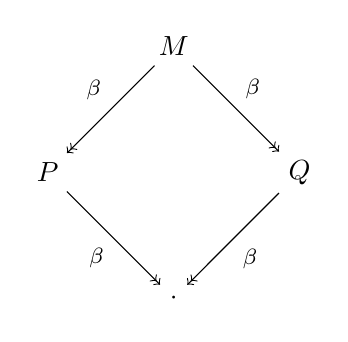
\begin{tikzpicture}[scale=0.8]
        \node (M) at (0, 0) {$M$};
        \node (P) at (-2, -2) {$P$};
        \node (Q) at (2, -2) {$Q$};
        \node (X) at (0, -4) {$\cdot$};
        \draw[->>] (M) to node[above left] {\footnotesize$\beta$} (P);
        \draw[->>] (M) to node[above right] {\footnotesize$\beta$} (Q);
        \draw[->>] (P) to node[below left] {\footnotesize$\beta$} (X);
        \draw[->>] (Q) to node[below right] {\footnotesize$\beta$} (X);
    \end{tikzpicture}
    \caption{Własność rombu relacji $\toto_\beta$.}
    \label{fig:church-rosser}
\end{figure}

Prostym wnioskiem z tego twierdzenia jest fakt, że każdy term ma co najwyżej jedną postać normalną, to znaczy pozbawioną $\beta$-redeksów.
Dlaczego \emph{co najwyżej}, a nie \emph{dokładnie}? Na przykład term
\[ \symbf{\Omega} \coloneqq \left(\lambda x\ldotp xx\right)\left(\lambda x\ldotp xx\right) \]
posiada tylko jeden $\beta$-redeks, którego redukcja prowadzi do termu $\symbf{\Omega}$ (co Czytelnik raczy sprawdzić), czyli $\symbf{\Omega} \to_\beta \symbf{\Omega}$. Term $\symbf{\Omega}$ nie ma więc postaci normalnej.

\begin{remark}[Rachunek lambda jako teoria równościowa]
    Rachunek lambda z $\beta$-redukcją można potraktować jako teorię równościową (zwaną teorią $\lambda\beta$), czyli zbiór formuł zamknięty ze względu na reguły wnioskowania. Czytelnik zainteresowany logiką formalną może zastanowić się, jakie reguły wnioskowania są potrzebne oraz co daje nam opisana niżej $\eta$-redukcja (teoria $\lambda\beta\eta$).
\end{remark}

\subsubsection*{Eta-redukcja}

\vocab{$\eta$-redukcja} to taka relacja $\to_\eta$ w zbiorze termów $\Lambda$, że $M \to_\eta N$, gdy \vocab{$\eta$-redeks} postaci $\lambda x\ldotp Px$ w termie M zostaje zastąpiony przez $P$ w termie $N$, zakładając $x \notin \FV(P)$.

Tak jak poprzednio, dokmnięcie przechodnio-zwrotne relacji $\to_\eta$ oznaczamy przez $\toto_\eta$. Ponadto, sumę relacji $\to_\beta$ i $\to_\eta$ oznaczamy przez $\to_{\beta\eta}$, a jej domknięcie przechodnio-zwrotne przez $\toto_{\beta\eta}$.

\todo[inline]{Konfuentność $\to_\eta$?}

W tym miejscu kończymy krótkie wprowadzenie do rachunku lambda, chociaż nie można powiedzieć, że temat został wyczerpany chociaż w najmniejszym stopniu. Zaintrygowany Czytelnik może przeczytać więcej o kombinatorach punktu stałego, drzewach Böhma czy wreszcie reprezentowaniu obliczeń maszyny Turinga za pomocą rachunku lambda.

\subsubsection*{Kilka ćwiczeń}

W poniższych ćwiczeniach warto wykorzystać poznany wcześniej kombinator $\symbf{\Omega}$ lub kombinator $\symbf{Y} \coloneqq \lambda f\ldotp (\lambda x\ldotp f (xx)) (\lambda x\ldotp f (xx))$ o tej ciekawej własności, że dla każdego termu $F \in \Lambda$ zachodzi
\[ F(\symbf{Y}(F)) =_\beta \symbf{Y}(F). \]

\begin{problem}
    Znajdź term $P$ taki, że $Px =_\beta P$.
\end{problem}

\begin{problem}
    Znajdź term $P$ taki, że $Px =_\beta xP$.
\end{problem}

\subsection{Teoria typów}

Zajmiemy się teraz sposobem typowania rachunku lambda wprowadzonym przez Alonzo Churcha (istnieje również alternatywna, równie popularna, wersja wprowadzona przez Haskella Curry'ego).



Teoria zbiorów służy za podstawę matematyki, ponieważ oferuje informacje semantyczne, np.
\[ 7 \in \left\{n \in \NN \mid \forall a \in \NN, a^n \equiv a \pmod{n} \right\}. \]
Ze skonstruowanych w ten sposób zbiorów łatwo odczytać interesujące nas własności, trudniej jednak dowieść ich prawdziwości.
Z drugiej strony teoria typów oferuje (uboższe na pierwszy rzut oka) informacje syntaktyczne, np.
\[ 1 + (2 \cdot 3) : \NN, \]
za to nie potrzebuje \emph{dowodu}, a jedynie \emph{obliczenia} zgodnie z danymi regułami.

\subsubsection*{Izomorfizm Curry'ego-Howarda}

Izomorfizm Curry'ego-Howarda to twierdzenie, które łączy logikę i teorię typów.
Mówi ono, że jeśli formułom logicznym przypiszemy odpowiednie typy, a dowodom tych formuł przypiszemy odpowiednie termy, to otrzymamy izomorfizm postaci:
\[ \text{formuła ma dowód} \iff \text{typ ma term}. \]
W ten sposób możemy przepisać formułę logiczną do postaci typu i udowodnić ją, konstruując term tego typu.
W tym właśnie procesie przydaje się oprogramowanie takie jak Lean.

\todo[inline]{Dokończyć opis izomorfizmu Curry'ego-Howarda oraz całą sekcję o teorii typów.}

\section{Podstawy dowodzenia w Lean}

\subsection{Środowisko}

Polecam używać VS Code z rozszerzeniem \textbf{Lean 4} lub Neovim z rozszerzeniem \textbf{lean.nvim}.
Aby rozpocząć pracę, należy stworzyć projekt za pomocą
\begin{minted}{bash}
lake new project-name math-lax
\end{minted}
który od razu dodaje Mathlib do wymaganych zależności.

\todo[inline]{wyjaśnić theorem, example, nawiasy klamrowe i okrągłe}

\subsection{Rachunek zdań i pierwsze taktyki}

\subsubsection*{Taktyki \texttt{intro}, \texttt{exact} i \texttt{apply}}

Jeśli cel dowodzenia znajduje się wśród założeń, to wystarczy go wskazać za pomocą taktyki \Lean{exact}. Jeśli cel jest w postaci \Lean{P → Q}, to możemy użyć taktyki \Lean{intro}, aby wprowadzić do dowodu założenie \Lean{P} i zmienić cel na \Lean{Q}.
\begin{minted}{lean4}
example {P : Prop} (h : P) : P := by
  exact h

example {P : Prop} : P → P := by
  intro h
  exact h
\end{minted}

Jeśli celem jest \Lean{Q}, a mamy wśród założeń \Lean{P → Q}, to możemy użyć taktyki \Lean{apply}, aby zmienić cel na \Lean{P}. Możemy stosować również aplikację znaną z (typowanego) rachunku lambda.
\begin{minted}{lean4}
example {P Q : Prop} (h₁ : P → Q) (h₂ : P) : Q := by
  apply h₁
  exact h₂

example {P Q : Prop} (h₁ : P → Q) (h₂ : P) : Q := by
  exact h₁ h₂
\end{minted}

\subsubsection*{Koniunkcja i alternatywa}

W Lean istnieje struktura \Lean{And}, której jedynym konstrukturem jest
\centerLean[.]{And.intro {a b : Prop} (left : a) (right : b) : a ∧ b}
Jako że \Lean{And.intro} ma typ \Lean{a → b → a ∧ b}, to świetnie nadaje się do użycia z \Lean{apply}, które wprowadzi dwa cele (do rozwiązania jeden po drugim).

Jeśli chcemy w ten sposób użyć konstruktora dowolnej struktury, to możemy użyć taktyki \Lean{constructor}.

\begin{minted}{lean4}
example {P Q : Prop} (hp : P) (hq : Q) : P ∧ Q := by
  apply And.intro
  · exact hp
  · exact hq

example {P Q : Prop} (hp : P) (hq : Q) : P ∧ Q := by
  constructor
  · exact hp
  · exact hq

example {P Q : Prop} (h : P ∧ Q) : P := by
  exact h.left
\end{minted}

Podobnie istnieje struktura \Lean{Or}, której konstruktorami są
\centerLean{inl {a b : Prop} (h : a) : a ∨ b}
oraz
\centerLean[.]{inr {a b : Prop} (h : b) : a ∨ b}
Aby ich użyć, skorzystamy z taktyki \Lean{cases} lub \Lean{rcases} (które rekurencyjnie wywołuje \Lean{cases} zgodnie z podanym wzorem).
\begin{minted}{lean4}
example {P Q R : Prop} (hpq : P ∨ Q) (hpr : P → R) (hqr : Q → R) : R := by
  cases hpq with
  | inl hp =>
    apply hpr
    exact hp
  | inr hq =>
    apply hqr
    apply hq

example {P Q R : Prop} (hpq : P ∨ Q) (hpr : P → R) (hqr : Q → R) : R := by
  rcases hpq with hp | hq
  · apply hpr
    exact hp
  · apply hqr
    apply hq
\end{minted}

Taktyka \Lean{rcases} może się przydać również przy koniunkcjach i bardziej złożonych zdaniach, na przykład:
\begin{minted}{lean4}
example {P Q R S : Prop} (h : S ∧ R ∧ P ∨ S ∧ (Q ∧ R)) : R := by
  rcases h with ⟨_, hr, _⟩ | ⟨_, ⟨_, hr⟩⟩
  · exact hr
  · exact hr
\end{minted}

Jeśli alternatywa jest naszym celem, a nie założeniem, to przydatne będą taktyki \Lean{left} i \Lean{right}.

\begin{minted}{lean4}
example {P Q : Prop} (h : P) : P ∨ Q := by
  left
  exact h
\end{minted}

\begin{remark}
    Bardziej dokładnie, taktyka \Lean{constructor} używa pierwszego pasującego konstruktora struktury, a taktyki \Lean{left} i \Lean{right} używają odpowiednio pierwszego i drugiego konstruktora struktury, która ma dokładnie dwa konstruktory. Nie są one przypisane do struktur \Lean{And} i \Lean{Or}. W szczególności, zamiast \Lean{left} zawsze można używać \Lean{constructor}, ale sensowność takiego działania pozostawiamy do oceny Czytelnikowi.
\end{remark}

\subsubsection*{Nawiasowanie}

\subsubsection*{Negacja}

\subsubsection*{Taktyki \texttt{assumption}, \texttt{contradiction}, \texttt{trivial} oraz \texttt{<;>}}

Poniższy przykład (reguła \textit{modus tollendo ponens}) Czytelnik powinien już być w stanie zrozumieć. Pokażemy, jak udowodnić go trochę prościej.
\begin{minted}{lean4}
example {P Q : Prop} (h : P ∨ Q) (not_p : ¬P) : Q := by
  rcases h with hp | hq
  · apply False.elim (not_p hp)
  · exact hq
\end{minted}

Zamiast \Lean{exact hq} możemy użyć taktyki \Lean{assumption}, która sprawdza, czy cel jest wśród założeń (nie musimy go wskazywać). Zamiast \Lean{apply False.elim} możemy użyć taktyki \Lean{contradiction}, która sprawdza, czy wśród założeń znajdują się dwa trywialne sprzeczne stwierdzenia.
\begin{minted}{lean4}
example {P Q : Prop} (h : P ∨ Q) (not_p : ¬P) : Q := by
  rcases h with hp | hq
  · contradiction
  · assumption
\end{minted}

Jeśli nie używamy wprowadzonych założeń (w przykładzie \Lean{hp} i \Lean{hq}), to nie musimy ich nazywać -- dalej będą one dostępne dla taktyk \Lean{assumption} i \Lean{contradiction}.
\begin{minted}{lean4}
example {P Q : Prop} (h : P ∨ Q) (not_p : ¬P) : Q := by
  cases h
  · contradiction
  · assumption
\end{minted}

Istnieje również taktyka \Lean{trivial}, która próbuje rozwiązać cel używając kilku prostych taktyk, jak \Lean{assumption}, \Lean{contradiction} czy \Lean{rfl} (użyteczna przy równościach).
\begin{minted}{lean4}
example {P Q : Prop} (h : P ∨ Q) (not_p : ¬P) : Q := by
  cases h
  · trivial
  · trivial
\end{minted}

Jeśli chcemy użyć tej samej taktyki dla różnych przypadków, to możemy użyć \Lean{<;>} w następujący sposób:
\begin{minted}{lean4}
example {P Q : Prop} (h : P ∨ Q) (not_p : ¬P) : Q := by
  cases h <;> trivial
\end{minted}


\end{document}
